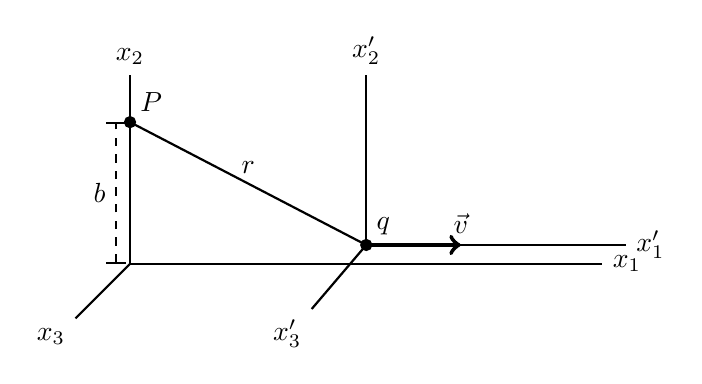
\begin{tikzpicture}[thick, scale=0.60]
	% A caceta dos eixos...
		\draw[-] (0,0) --  (10,0)node[right]{$x_1$};
		\draw[-] (0,0) -- (0,4) node[above]{$x_2$};
		\draw[-] (0,0) -- (0,0,3) node[below left]{$x_3$};
		\draw[-] (5,0.4) -- (10.5,0.4) node[right]{$x'_1$};
		\draw[-] (5,0.4) -- (5,4) node[above]{$x' _2$};
		\draw[-] (5,0.4) -- (5,0.2,3) node[below left]{$x'_3$};

	% A caceta dos desenhos que importam
		\filldraw (5,0.4) circle(3pt) node[above right] {$q$};
		\filldraw (0,3) circle(3pt) node[above right] {$P$};
		\draw (0,3) -- node[above]{$r$} (5,0.4);
		\draw[|-|,dashed] (-0.3,0) -- node[fill=white,left]{$b$} (-0.3,3);
		\draw[->,ultra thick] (5,0.4) -- (7,0.4) node[above]{$\vec{v}$};
\end{tikzpicture}

